\begin{figure}
	\centering
	\begin{tikzpicture}[
		every node/.style = {
			text width = 0.275\textwidth,
			inner sep = 0pt,
			outer sep = 0pt,
		},
		node distance = 1mm and 1mm
	]%
		% Row 1
		\node (d1) {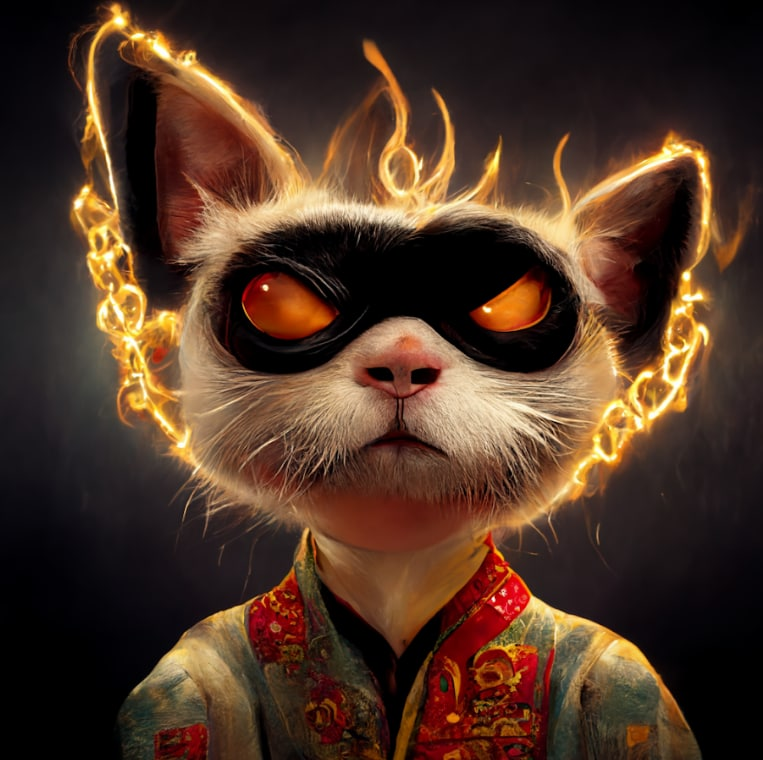
\includegraphics[width=\linewidth]{img/devilish-1}};
		\node [right = of d1] (d2) {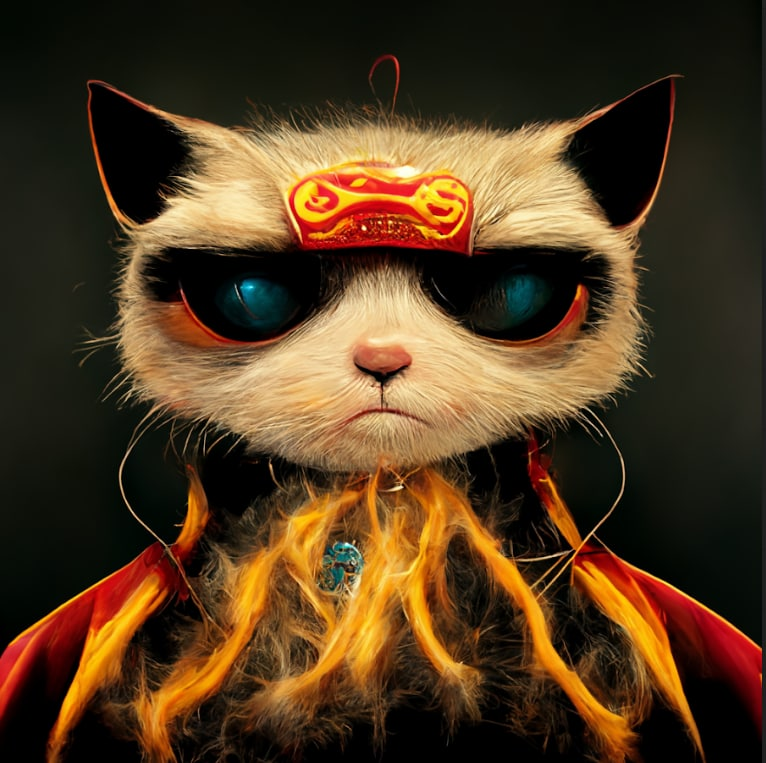
\includegraphics[width=\linewidth]{img/devilish-2}};
		% Row 2
		\node [below = of d1] (kf1) {
\includegraphics[width=\linewidth]{img/kung_fu-1}};
		\node [below = of d2] (kf2) {
\includegraphics[width=\linewidth]{img/kung_fu-2}};
	\end{tikzpicture}
	\caption{The NFT appraisal model can be run ``in reverse'', as statistically-optimal generative models for a given set of traits and art styles. To be released as several collections on mainnet. Why cats and not frogs? Because we're saving the best for last\ldots}%
	\label{fig:reverse}
\end{figure}

